\documentclass{article}

\usepackage{microtype}
\usepackage{graphicx}
\usepackage{booktabs}
\usepackage{hyperref}

% Default to the anonymous review format.
% Switch to \usepackage[accepted]{icml2026} for the camera-ready version.
\usepackage{icml2026}

\usepackage{amsmath,amssymb,amsthm,mathtools}
\usepackage{enumitem}
\usepackage[capitalize,noabbrev]{cleveref}

\theoremstyle{plain}
\newtheorem{theorem}{Theorem}[section]
\newtheorem{proposition}[theorem]{Proposition}
\newtheorem{lemma}[theorem]{Lemma}
\newtheorem{corollary}[theorem]{Corollary}
\theoremstyle{definition}
\newtheorem{assumption}{Assumption}
\newtheorem{definition}[theorem]{Definition}
\theoremstyle{remark}
\newtheorem{remark}[theorem]{Remark}

\newcommand{\HM}{\mathrm{HM}}
\newcommand{\AM}{\mathrm{AM}}
\newcommand{\Var}{\mathrm{Var}}
\newcommand{\E}{\mathbb{E}}
\newcommand{\proj}{\operatorname{proj}}
\DeclareMathOperator{\diag}{diag}
\DeclareMathOperator{\OS}{OS}
\newcommand{\placeholderfigure}[3]{
  \begin{figure}[t]
  \centering
  \fbox{
    \begin{minipage}{0.94\linewidth}
    \small
    \textbf{#1}
\par\vspace{0.5em}
    #2
    \end{minipage}
  }
  \caption{#3}
  \end{figure}
}

\icmltitlerunning{Evidence-Weighted and Opponent-Shaped Policy Gradient}

\begin{document}

\twocolumn[
\icmltitle{Evidence-Weighted and Opponent-Shaped Policy Gradient with Composed Convergence Guarantees}

\begin{icmlauthorlist}
\icmlauthor{Yevhen Shcherbinin}{bt,lse}
\icmlauthor{Maxim Kalpin}{bt,jku}
\icmlauthor{Arina Redina}{bristol,bt}
\icmlauthor{Vlad Kochetov}{bt,opnu}
\end{icmlauthorlist}

\icmlaffiliation{bt}{Bloomsbury Technology, London, United Kingdom}
\icmlaffiliation{lse}{London School of Economics and Political Science, London, United Kingdom}
\icmlaffiliation{jku}{Johannes Kepler University Linz, Linz, Austria}
\icmlaffiliation{bristol}{University of Bristol, Bristol, United Kingdom}
\icmlaffiliation{opnu}{Odessa Polytechnic National University, Odesa, Ukraine}
\icmlcorrespondingauthor{Yevhen Shcherbinin}{eugene.shcherbinin@bloomsburytech.com}
\icmlkeywords{multi-agent reinforcement learning, policy gradient, stochastic games}

\vskip 0.3in
]

\printAffiliationsAndNotice{}

\begin{abstract}
Policy-gradient methods in general stochastic games now admit local convergence guarantees to stable Nash policies, but two practical weaknesses remain. First, agents often learn from observations of uneven quality, so equal-weight updates let the noisiest gradients dominate the joint dynamics. Second, even when a stable Nash policy exists, the basin of attraction may be small, making convergence sensitive to initialisation. We study two modifications that address these weaknesses without leaving the convergence regime of \citet{giannou2022convergence}. Evidence-weighted policy gradient (EW-PG) rescales each agent's update by an inverse-variance evidence weight and reduces the effective gradient variance by a factor $\HM(V)/\AM(V)\leq 1$. Opponent-shaped policy gradient (LOLA-PG) adds a one-step opponent-shaping term and, under an annealed shaping schedule, preserves local convergence, while under constant shaping it enlarges the local attraction region when the shaping Jacobian satisfies a spectral reinforcement condition. Our main contribution is a composition result that separates these two regimes cleanly: annealed EW-LOLA-PG preserves the variance improvement and convergence rate, and the corresponding frozen-weight constant-shaping dynamics inherit the local geometric gain. The draft is supported by completed matrix-game, basin-mapping, and persona-conditioned iterated-game runs, with explicit placeholder slots reserved only for the remaining workshop figures.
\end{abstract}

\section{Introduction}

Policy-gradient learning in multi-agent systems long lacked trajectory-level convergence guarantees outside narrow game classes. \citet{giannou2022convergence} changed that picture by proving local convergence to stable Nash policies in general stochastic games under a stable second-order condition. That theorem gives a clean baseline, but it does not by itself solve two problems that matter in practice. The first is heteroskedasticity across agents: gradient estimators can have sharply different variances because agents observe different histories and occupy different informational positions in the game. The second is geometric: local convergence only helps when initialisation lands in the attraction region of the target equilibrium, and that region may be small.

This paper studies two modifications that target those problems on orthogonal axes. Evidence-weighted policy gradient (EW-PG) scales each agent's update by a Keynesian evidence weight proportional to the inverse of its gradient variance; we show this yields an $\HM(V)/\AM(V)\le 1$ improvement in the convergence constant while preserving the Giannou rate exponent (Theorems~\ref{thm:ew-var},~\ref{thm:ew-conv}). Learning with Opponent-Learning Awareness (LOLA) takes a different route. \citet{foerster2018lola} introduced a shaping term that anticipates how the current agent changes the opponent's next update. The original paper showed strong behavioural effects in iterated prisoner's dilemma and convergence to Nash play in repeated matching pennies, but it did not provide a general local convergence theorem for stochastic games. We close that gap by separating two claims that are often bundled together: annealed shaping preserves the Giannou rate (Theorem~\ref{thm:lola-rate}), while constant shaping enlarges the local attraction region under a spectral reinforcement condition (Theorem~\ref{thm:lola-basin}).

The main claim of this paper is that these two improvements compose cleanly, but that conclusion is not automatic. Evidence weights multiply the same coordinates that LOLA shapes, so they could in principle damp the shaping benefit, distort the favourable Jacobian symmetry, or couple online weight-estimation noise to the shaping bias. The composition result matters because the local analysis separates the mechanisms cleanly: under annealing, evidence weighting changes the martingale variance constant while LOLA changes only the bias budget; under frozen weights and constant shaping, the same weighted Jacobian determines the local geometry. No additional mixed term is needed in either regime.

We make four contributions. First, we restate the \citet{giannou2022convergence} framework in the minimal quantitative form we will sharpen (Section~\ref{sec:prelim}). Second, we isolate the EW-PG result as a variance-reduction theorem with preserved local convergence (Theorems~\ref{thm:ew-var}--\ref{thm:ew-conv}). Third, we isolate the LOLA-PG result as a rate-preserving opponent-shaping method with a separate basin-enlargement theorem for the constant-shaping local dynamics (Theorems~\ref{thm:lola-rate}--\ref{thm:lola-basin}). Fourth, we state and prove a composition theorem for annealed EW-LOLA-PG, together with the corresponding frozen-weight geometric corollary (Theorem~\ref{thm:ewlola} and Proposition~\ref{prop:ewlola-geometry}; proof roadmap in Appendix~\ref{app:proof}).

\section{Preliminaries}\label{sec:prelim}

\subsection{Stochastic game and policy gradient}

We work with finite stochastic games in the tabular episodic setting. A game is a tuple
\begin{equation}\label{eq:game}
\mathcal{G} = (N,\mathcal{S},\{\mathcal{A}_i\}_{i\in N},\{R_i\}_{i\in N},P,\rho,\gamma_{\mathrm{disc}}),
\end{equation}
where $N=\{1,\ldots,N\}$ is the set of agents, $\mathcal{S}$ a finite state space, $\mathcal{A}_i$ agent $i$'s finite action set, $R_i:\mathcal{S}\times\prod_j \mathcal{A}_j\to\mathbb{R}$ its reward, $P:\mathcal{S}\times\prod_j\mathcal{A}_j\to\Delta(\mathcal{S})$ the transition kernel, $\rho\in\Delta(\mathcal{S})$ the initial-state distribution, and $\gamma_{\mathrm{disc}}\in[0,1)$ the discount factor. Each agent chooses a stationary Markov policy $\pi_i\in\Pi_i := \Delta(\mathcal{A}_i)^{|\mathcal{S}|}$, and the joint policy lies in
\[
\Pi := \prod_{i\in N}\Pi_i \;\subset\; \mathbb{R}^d, \qquad d := \sum_{i\in N}|\mathcal{A}_i|\cdot|\mathcal{S}|.
\]
For each agent $i$, let $J_i(\pi) := \E_{\pi,\rho}\!\left[\sum_{t\ge 0}\gamma_{\mathrm{disc}}^t R_i(s_t,a_t)\right]$ be the expected discounted return, and
\begin{equation}\label{eq:grad}
\begin{aligned}
v_i(\pi) &:= \nabla_{\pi_i}J_i(\pi),\\
v(\pi) &:= (v_i(\pi))_{i\in N},
\end{aligned}
\end{equation}
the per-agent and joint policy gradients. The projected joint policy-gradient update is
\begin{equation}\label{eq:pg}
\pi_{n+1} = \proj_{\Pi}\!\bigl(\pi_n + \gamma_n \hat v_n\bigr), \qquad \gamma_n := \frac{\gamma}{(n+m)^p},
\end{equation}
where $\hat v_n$ is a stochastic gradient estimator (for instance REINFORCE), $\gamma>0$ and $p\in(1/2,1]$ are fixed constants, and $m\ge 1$ is a deterministic offset whose only purpose is to keep $\gamma_1$ uniformly bounded away from $0$ and $\infty$ (it does not affect any asymptotic conclusion). Let $\mathcal{F}_n := \sigma(\pi_0,\hat v_0,\ldots,\hat v_{n-1})$ denote the natural filtration of the algorithm.

\subsection{Stable Opponent-Sensitive (SOS) Nash equilibrium}

\begin{definition}[SOS Nash equilibrium]\label{def:sos}
A joint policy $\pi^\ast\in\Pi$ is a \emph{Stable Opponent-Sensitive (SOS) Nash equilibrium} with parameters $(\mu,\rho_{\mathrm{nbd}})$, where $\mu>0$ and $\rho_{\mathrm{nbd}}>0$, if $v(\pi^\ast)=0$ and, for every $\pi\in\Pi$ with $\|\pi-\pi^\ast\|<\rho_{\mathrm{nbd}}$,
\begin{equation}\label{eq:sos}
\langle v(\pi),\,\pi-\pi^\ast\rangle \;\le\; -\mu\,\|\pi-\pi^\ast\|^{2}.
\end{equation}
\end{definition}

\begin{remark}[Relationship to prior definitions]
Condition~\eqref{eq:sos} is the local strong-monotonicity refinement used by \citet{giannou2022convergence} to obtain quantitative contraction. We use the SOS name to distinguish it from the weaker notion of a Nash point where $v$ merely vanishes, because the \emph{strict} inequality~\eqref{eq:sos} carries a uniform drift constant that the later analysis tracks explicitly.
\end{remark}

\subsection{Stochastic-approximation conditions and baseline rate}

We restate the local convergence rate in a form the rest of the paper can build on. All subsequent theorems operate within the quantitative version below. Fix exponents $\ell_b,\ell_\sigma\ge 0$ and assume:
\begin{enumerate}[label=\textup{(B\arabic*)},leftmargin=1.8em,itemsep=0.2em]
  \item \textup{(Bias).} $\|\E[\hat v_n-v(\pi_n)\mid\mathcal{F}_n]\|\le B_n$ with $B_n = O(n^{-\ell_b})$;
  \item \textup{(Variance).} $\E\!\left[\|\hat v_n-\E[\hat v_n\mid\mathcal{F}_n]\|^2\mid\mathcal{F}_n\right]\le \sigma_n^2$ with $\sigma_n^2 = O(n^{2\ell_\sigma})$;
  \item \textup{(Schedule).} $p+\min(\ell_b,\,p-2\ell_\sigma)>1$ and $2\gamma\mu>q$, where
  \[
    q := \min\!\bigl(\ell_b,\,p-2\ell_\sigma\bigr).
  \]
\end{enumerate}

\begin{proposition}[Baseline rate; specialization of {\citealp[Thm.\,1]{giannou2022convergence}}]\label{prop:giannou}
Let $\pi^\ast$ be an SOS Nash equilibrium with parameters $(\mu,\rho_{\mathrm{nbd}})$ and assume \textup{(B1)--(B3)}. For every $\varepsilon>0$ there exist $\delta(\varepsilon)>0$ and a measurable localization event $\mathcal{E}_\varepsilon\in\mathcal{F}_\infty$ with $\mathbb{P}[\mathcal{E}_\varepsilon]\ge 1-\varepsilon$ such that, conditional on $\pi_0$ lying in the $\delta(\varepsilon)$-neighbourhood of $\pi^\ast$ and on $\mathcal{E}_\varepsilon$ (which is the event that the iterates $\{\pi_n\}$ never leave the $\rho_{\mathrm{nbd}}$-neighbourhood of $\pi^\ast$), we have
\begin{equation}\label{eq:giannou}
\E\!\left[\|\pi_n-\pi^\ast\|^2 \,\big|\, \mathcal{E}_\varepsilon\right] \;=\; O\!\bigl(C/n^q\bigr),
\end{equation}
for a structural constant $C=C(\mu,\gamma,p,\ell_b,\ell_\sigma)>0$.
\end{proposition}

We will use~\eqref{eq:giannou} as a \emph{baseline}, not as a black box: the theorems below sharpen $C$ (via evidence weights) and enlarge the effective $\mu$ (via opponent shaping) without changing $q$.

\subsection{Harmonic and arithmetic means}

For a tuple $V=(V_1,\ldots,V_N)$ of strictly positive reals, define
\begin{equation}\label{eq:amhm}
\AM(V) := \frac{1}{N}\sum_{i=1}^N V_i, \qquad
\HM(V) := \Bigl(\frac{1}{N}\sum_{i=1}^N V_i^{-1}\Bigr)^{-1}.
\end{equation}
The AM--HM inequality $\HM(V)\le\AM(V)$ with equality iff all $V_i$ are equal will be invoked repeatedly \citep{HardyLittlewoodPolya1952}.

\section{Evidence-Weighted Policy Gradient}

\subsection{Setup}

In multi-agent learning the agents do not observe the game through equally informative histories. Some sit in stable information states with low-variance gradient estimates; others face noisier observations or more weakly identified best responses. Standard joint policy gradient ignores that heterogeneity: every agent receives the same global step-size even when its estimator is much noisier than the rest.

\begin{definition}[Keynesian evidence weights]\label{def:evw}
Let $V_{i,n} := \Var(\hat v_{i,n})$ be the per-agent gradient-estimator variance at iteration $n$, and define
\begin{equation}\label{eq:ewweights}
w_{i,n} := \frac{V_{\min,n}}{V_{i,n}}\in(0,1], \qquad V_{\min,n} := \min_{j\in N} V_{j,n}.
\end{equation}
Agents with the lowest variance receive weight $1$; noisier agents are downweighted proportionally. The \emph{evidence-weighted policy-gradient} (EW-PG) update is
\begin{equation}\label{eq:ew-update}
\pi_{i,n+1} = \proj_{\Pi_i}\!\bigl(\pi_{i,n} + \gamma_n\, w_{i,n}\, \hat v_{i,n}\bigr),
\end{equation}
with the same step size $\gamma_n$ as in~\eqref{eq:pg}.
\end{definition}

We state the theory for oracle (or locally frozen) variances $V_{i,n}$; the online estimator~\eqref{eq:hatsigma} below inherits the same guarantees in the limit of a growing window.

\begin{definition}[Online plug-in weights]\label{def:plugin}
Using a window of $M\in\mathbb{N}$ recent minibatch gradients $g_{i,k}$ with running mean $\bar g_{i,n}$, define
\begin{equation}\label{eq:hatsigma}
\begin{aligned}
\hat\sigma^2_{i,n}
&:= \frac{1}{M-1}\sum_{k=n-M+1}^{n}\|g_{i,k}-\bar g_{i,n}\|^2,\\
\hat w_{i,n}
&:= \frac{1/\hat\sigma^2_{i,n}}
{\max_{j\in N}\,1/\hat\sigma^2_{j,n}}.
\end{aligned}
\end{equation}
\end{definition}

\begin{proposition}[Consistency of plug-in weights]\label{prop:plugin}
Under strict local stationarity of $\{g_{i,k}\}_{k\ge k_0}$ with $\Var(g_{i,k})=V_i\in(0,\infty)$ and finite fourth moments, $\hat\sigma^2_{i,n}\to V_i$ almost surely as $M\to\infty$, and hence $\hat w_{i,n}\to w_i := V_{\min}/V_i$ almost surely.
\end{proposition}

\begin{proof}
Each $\hat\sigma^2_{i,n}$ is a sample variance of an ergodic sequence, which converges to $V_i$ almost surely by the ergodic theorem under the stated moment assumption. Continuity of the map $V\mapsto V_{\min}/V_i$ on $(0,\infty)^N$ lifts this to the weights.
\end{proof}

A full transient analysis of plug-in weights (with finite $M$ and a time-varying target) is deferred to future work; the convergence theorems below use oracle weights.

\subsection{Variance improvement}

The central algebraic ingredient is the weighted-variance identity, stated and proved in full.

\begin{lemma}[AM--HM variance improvement]\label{lem:amhm}
Let $V=(V_1,\ldots,V_N)$ be strictly positive and let $w_i := V_{\min}/V_i$ with $V_{\min} := \min_j V_j$. Then
\begin{equation}\label{eq:amhm-ratio}
\frac{\sum_{i=1}^N w_i^2\,V_i}{\sum_{i=1}^N V_i} \;=\; \frac{V_{\min}^2}{\HM(V)\cdot\AM(V)} \;\le\; \frac{\HM(V)}{\AM(V)} \;\le\; 1,
\end{equation}
with equality in the right inequality iff all $V_i$ are equal.
\end{lemma}

\begin{proof}
Substitute $w_i=V_{\min}/V_i$ to get $\sum_i w_i^2 V_i = V_{\min}^2 \sum_i V_i^{-1} = N V_{\min}^2/\HM(V)$. The standard (unweighted) denominator is $\sum_i V_i = N\AM(V)$. Their ratio equals $V_{\min}^2/[\HM(V)\AM(V)]$, the equality in~\eqref{eq:amhm-ratio}. Since $V_{\min}\le\HM(V)$ (the minimum is a lower bound for the harmonic mean), we have $V_{\min}^2\le V_{\min}\cdot\HM(V)\le\HM(V)^2$, giving the first inequality. The AM--HM inequality \citep[\S2.5]{HardyLittlewoodPolya1952} gives the second, with equality iff all $V_i$ are equal.
\end{proof}

\begin{theorem}[Variance improvement of EW-PG]\label{thm:ew-var}
Let $\sigma^2_{\mathrm{std}} := \sum_{i=1}^N V_i$ denote the joint-gradient variance of standard PG and $\sigma^2_w := \sum_{i=1}^N w_i^2\,V_i$ that of EW-PG with oracle weights $w_i=V_{\min}/V_i$. Then
\begin{equation}\label{eq:ewvar}
\sigma^2_w \;\le\; \frac{\HM(V)}{\AM(V)}\,\sigma^2_{\mathrm{std}} \;\le\; \sigma^2_{\mathrm{std}},
\end{equation}
with equality on the right iff all $V_i$ are equal.
\end{theorem}

\begin{proof}
Immediate from Lemma~\ref{lem:amhm} by multiplying through by $\sigma^2_{\mathrm{std}}$.
\end{proof}

\subsection{Convergence of EW-PG}

\begin{assumption}[Weighted SOS condition]\label{as:wsos}
There exist $\mu_W>0$ and a neighbourhood $\Omega\ni\pi^\ast$ such that, with $W^\ast := \diag(w_1^\ast,\ldots,w_N^\ast)$ the oracle weight matrix at $\pi^\ast$,
\begin{equation}\label{eq:wsos}
\langle W^\ast v(\pi),\,\pi-\pi^\ast\rangle \;\le\; -\mu_W\,\|\pi-\pi^\ast\|^2 \qquad \forall\pi\in\Omega.
\end{equation}
\end{assumption}

\begin{remark}
If $w_i^\ast\ge c>0$ for all $i$ and $\pi^\ast$ is SOS with constant $\mu$ (Definition~\ref{def:sos}), then~\eqref{eq:wsos} holds with $\mu_W\ge c\mu$ whenever the distortion $W^\ast$ is close to a scalar multiple of the identity. In general~\eqref{eq:wsos} is stated as a direct assumption because severe downweighting of a single agent can, in principle, lose monotonicity.
\end{remark}

\begin{theorem}[Convergence of EW-PG]\label{thm:ew-conv}
Assume \textup{(B1)--(B3)}, Definition~\ref{def:sos} for $(\mu,\rho_{\mathrm{nbd}})$, and Assumption~\ref{as:wsos}. Using oracle weights $w_{i,n}=V_{\min,n}/V_{i,n}$ in the update~\eqref{eq:ew-update}, the conclusion of Proposition~\ref{prop:giannou} holds with an improved constant:
\begin{equation}\label{eq:ew-conv}
\E\!\left[\|\pi_n-\pi^\ast\|^2 \,\big|\, \mathcal{E}_\varepsilon\right] \;=\; O\!\left(\frac{\HM(V)}{\AM(V)}\cdot\frac{C}{n^q}\right),
\end{equation}
where $V=(V_i)_{i\in N}$ are the (frozen) local gradient variances, $q=\min(\ell_b,p-2\ell_\sigma)$, and $C$ is the constant of Proposition~\ref{prop:giannou}.
\end{theorem}

\begin{proof}[Proof sketch]
The Lyapunov analysis of \citet{giannou2022convergence} yields a recursion of the form
\(
\E[V_{n+1}\mid\mathcal{F}_n]\le V_n(1-2\gamma_n\mu_W) + A_n^{(b)} + A_n^{(\sigma)},
\)
where $V_n=\|\pi_n-\pi^\ast\|^2$, $A_n^{(b)}=O(n^{-(p+2\ell_b)})$ is the bias forcing, and $A_n^{(\sigma)}=O(n^{-(2p-2\ell_\sigma)})$ is the variance forcing. Under (B3), the discrete Gr\"onwall bound gives the rate $O(n^{-q})$. Substituting the oracle weights replaces the variance forcing $A_n^{(\sigma)}$ by $[\HM(V)/\AM(V)]\,A_n^{(\sigma)}$ via Lemma~\ref{lem:amhm}, and this factor propagates into the leading constant. A full proof appears as the specialization of Theorem~\ref{thm:ewlola} (Appendix~\ref{app:proof}) with $\lambda=0$.
\end{proof}

EW-PG is a residual step-allocation rule, not a replacement for standard variance-reduction tools. Counterfactual baselines such as COMA \citep{foerster2018coma} and optimal-baseline analyses for MARL policy gradients \citep{kuba2022variance} reduce each agent's \emph{own} estimator variance using richer conditioning. EW addresses a different question: given residual estimator-variance heterogeneity across agents, how should the joint update allocate trust across them? Larger rollout budgets can also equalize variances, but that raises sample cost and may be infeasible under asymmetric observation channels. EW is therefore orthogonal to critics, baselines, and larger batch sizes rather than a substitute for them.

\section{Opponent-Shaping Policy Gradient}

\subsection{The LOLA correction and its annealed schedule}

\citet{foerster2018lola} introduced Learning with Opponent-Learning Awareness to account for the fact that agent $i$'s own update changes the opponent's next update. In its simplest one-step form, the per-agent shaping term is
\begin{equation}\label{eq:os}
\OS_i(\pi) := \sum_{j\neq i}\frac{\partial R_i}{\partial \theta_j'}\,\frac{\partial \theta_j'}{\partial \theta_i}, \qquad \theta_j' := \theta_j - \eta_j\,\nabla_{\theta_j}R_j,
\end{equation}
where $\theta_j'$ is agent $j$'s anticipated one-step update with learning rate $\eta_j>0$. We write $\OS(\pi) := (\OS_i(\pi))_{i\in N}\in\mathbb{R}^d$ for the joint shaping field.

\begin{definition}[Annealed LOLA-PG]\label{def:lolapg}
Fix $\lambda>0$ and $r>1-p$, and define the \emph{annealed shaping coefficient}
\begin{equation}\label{eq:lambda-n}
\lambda_n := \frac{\lambda}{(n+m)^r}.
\end{equation}
The annealed LOLA-PG update is
\begin{equation}\label{eq:lola-update}
\pi_{i,n+1} := \proj_{\Pi_i}\!\bigl(\pi_{i,n} + \gamma_n\,(\hat v_{i,n} + \lambda_n\,\OS_{i,n})\bigr),
\end{equation}
where $\OS_{i,n}$ is a (possibly stochastic) estimator of $\OS_i(\pi_n)$ with bias satisfying condition (B1) with the same exponent $\ell_b$.
\end{definition}

The following theorem is about the Jacobian of the one-step field $\OS$ defined by~\eqref{eq:os}; it makes no claim about multi-step meta-gradients such as Meta-MAPG \citep{kim2021meta}, which differentiate through longer update chains and therefore study a richer object. The present claim is narrower: the one-step LOLA field already has a local Jacobian whose symmetric part can improve contraction near an SOS Nash equilibrium.

\subsection{Rate preservation}

\begin{theorem}[Annealed LOLA preserves convergence]\label{thm:lola-rate}
Assume \textup{(B1)--(B3)}, Definition~\ref{def:sos} for $\pi^\ast$ with $(\mu,\rho_{\mathrm{nbd}})$, and that the LOLA estimator $\OS_n$ satisfies $\|\E[\OS_n\mid\mathcal{F}_n] - \OS(\pi_n)\|=O(n^{-\ell_b})$ with $\|\OS_n\|$ square-integrable and uniformly bounded on compact subsets of $\Pi$. Let $\lambda_n$ be the annealed coefficient~\eqref{eq:lambda-n} with $r>1-p$. Then the update~\eqref{eq:lola-update} converges to $\pi^\ast$ at the same rate exponent $q=\min(\ell_b,p-2\ell_\sigma)$ as standard PG: the conclusion of Proposition~\ref{prop:giannou} holds unchanged.
\end{theorem}

\begin{proof}[Proof sketch]
The shaping term adds a bias of magnitude $\lambda_n\|\OS(\pi_n)-\OS(\pi^\ast)\| = O(\lambda_n\|\pi_n-\pi^\ast\|)$ together with an $O(\lambda_n n^{-\ell_b})$ estimator bias. Aggregating: the \emph{augmented} bias $b_n+\lambda_n\OS_n^{\mathrm{bias}}$ in (B1) is $O(n^{-\min(\ell_b,r)})$. The schedule condition $r>1-p$ yields $p+\min(\ell_b,r)>1$, which is exactly the summability condition in the martingale step of Proposition~\ref{prop:giannou}. Hence $q$ is unchanged. The full recursion appears in Appendix~\ref{app:proof}.
\end{proof}

\subsection{Basin enlargement}

\begin{definition}[Shaping Hessian]\label{def:hessian}
Let $H := \nabla_\pi \OS(\pi^\ast)\in\mathbb{R}^{d\times d}$ denote the Jacobian of the joint shaping field at $\pi^\ast$, and let $S_H := (H+H^\top)/2$ be its symmetric part.
\end{definition}

\begin{assumption}[Shaping expansion]\label{as:expand}
There exists a neighbourhood $\Omega\ni\pi^\ast$ such that
\(
\OS(\pi) = H(\pi-\pi^\ast) + \xi(\pi) \text{ with } \|\xi(\pi)\| = O(\|\pi-\pi^\ast\|^2)
\)
for all $\pi\in\Omega$.
\end{assumption}

\begin{assumption}[Spectral reinforcement]\label{as:spec}
$S_H\preceq 0$ in the PSD order, with largest eigenvalue $\lambda_{\max}(S_H) = -\mu_H\le 0$.
\end{assumption}

\begin{theorem}[Basin enlargement under spectral reinforcement]\label{thm:lola-basin}
Under Assumptions~\ref{as:expand}--\ref{as:spec}, LOLA-PG with \emph{constant} shaping $\lambda_n\equiv\lambda$ improves the local drift constant from $\mu$ to
\begin{equation}\label{eq:musi-lola}
\mu_{\mathrm{LOLA}} := \mu + \lambda\mu_H \;\ge\; \mu,
\end{equation}
strictly whenever $\mu_H>0$.
\end{theorem}

\begin{proof}[Proof sketch]
Under Assumption~\ref{as:expand}, $\langle\OS(\pi),\pi-\pi^\ast\rangle = (\pi-\pi^\ast)^\top H(\pi-\pi^\ast)+O(\|\pi-\pi^\ast\|^3)$. The antisymmetric part of $H$ vanishes in this quadratic form, so $(\pi-\pi^\ast)^\top H(\pi-\pi^\ast) = (\pi-\pi^\ast)^\top S_H(\pi-\pi^\ast) \le -\mu_H\|\pi-\pi^\ast\|^2$ by Assumption~\ref{as:spec}. Adding $\lambda$ times this drift to the SOS inequality~\eqref{eq:sos} yields~\eqref{eq:musi-lola}. The annealed statement follows from Abel summation applied to $\sum_n\gamma_n\lambda_n$; convergence of that series uses $p+r>1$.
\end{proof}

The spectral condition is restrictive but not opaque. Two sufficient cases match the usual LOLA intuition: (i) in two-player zero-sum games the base gradient field has a strong antisymmetric rotational component that shaping converts into contraction; (ii) locally negative cross-Hessians favour reinforcement because the agents' objectives pull against one another in a way that the shaping term stabilizes. Potential games typically do \emph{not} benefit: if the base field is already locally contractive and mostly symmetric, there is little rotational structure for LOLA to exploit. This domain dependence motivates the competitive-game focus (matching pennies, rock--paper--scissors) of the basin-enlargement experiment in Section~\ref{sec:experiments}.

\begin{remark}[Why annealing and basin enlargement should be discussed separately]
Theorem~\ref{thm:lola-basin} is a statement about the local geometry of the \emph{constant}-shaping field. Under annealing, $\lambda_n\to 0$, so the extra drift vanishes asymptotically. Annealing is therefore the right regime for exact convergence, while constant shaping is the right regime for understanding how opponent shaping alters the nearby vector field. We keep both statements because the paper needs both kinds of information, but they answer different questions.
\end{remark}

\begin{remark}[Local versus global basin]
Theorem~\ref{thm:lola-basin} does not yield a closed-form volume for the attraction basin. Its content is local: a larger drift margin lets the Lyapunov argument of Proposition~\ref{prop:giannou} absorb higher-order remainders on a weakly larger neighbourhood. The empirical question is initialization sensitivity near $\pi^\ast$, not a global measure of basin size.
\end{remark}

\section{Composition: EW-LOLA-PG}\label{sec:composition}

We now combine the two modifications. Let
\(
W_n := \diag(w_{1,n},\ldots,w_{N,n})
\)
be the local evidence-weight matrix. The EW-LOLA-PG update is
\begin{equation}\label{eq:ewlola-update}
\pi_{i,n+1}
=
\proj_{\Pi_i}\!\Bigl(
\pi_{i,n}
+ \gamma_n\,w_{i,n}\bigl(\hat v_{i,n}+\lambda_n\,\OS_{i,n}\bigr)
\Bigr).
\end{equation}
This update is applied for each $i\in N$.

We state the composition theorem under a minimal, explicit assumption list. Assumptions \textup{(A1)--(A7)} generalize Assumption~\ref{as:wsos}, Assumptions~\ref{as:expand}--\ref{as:spec}, and (B1)--(B3) to the composed setting.

\begin{assumption}[Composed hypotheses]\label{as:composition}
There exist constants $\mu_W>0$, $\tilde\mu_H\ge 0$, $c>0$, $C_v<\infty$, and a neighbourhood $\Omega\ni\pi^\ast$ such that the following hold for all $\pi\in\Omega$, $n\ge 1$, and $i\in N$:
\begin{enumerate}[label=\textup{(A\arabic*)},leftmargin=2.0em,itemsep=0.15em]
  \item \textup{(Weighted SOS).} $\langle W^\ast v(\pi),\,\pi-\pi^\ast\rangle \le -\mu_W\|\pi-\pi^\ast\|^2$.
  \item \textup{(Bias).} $\|\E[\hat v_n-v(\pi_n)\mid\mathcal{F}_n]\|\le B_n$ with $B_n=O(n^{-\ell_b})$.
  \item \textup{(Variance).} $\E[\|\hat v_{i,n}-\E[\hat v_{i,n}\mid\mathcal{F}_n]\|^2\mid\mathcal{F}_n]\le V_{i,n}$ with $V_{i,n}=O(n^{2\ell_\sigma})$.
  \item \textup{(Shaping expansion).} $\OS(\pi) = H(\pi-\pi^\ast)+\xi(\pi)$ with $\|\xi(\pi)\|=O(\|\pi-\pi^\ast\|^2)$, and $v$ is $C_v$-Lipschitz on $\Omega$.
  \item \textup{(Weighted spectral reinforcement).} With $H_W := W^\ast H$ and $S_{H,W} := (H_W+H_W^\top)/2$, we have $S_{H,W}\preceq 0$ and $\lambda_{\max}(S_{H,W})=-\tilde\mu_H$.
  \item \textup{(Weight convergence).} $W_n\to W^\ast$ with $\|W_n-W^\ast\|=O(\|\pi_n-\pi^\ast\|)$ and $w_{i,n}^\ast\ge c>0$ for all $i$.
  \item \textup{(Schedule).} $r>1-p$ and $2\gamma\mu_W > q$, where $q := \min(\ell_b,\,p-2\ell_\sigma)$.
\end{enumerate}
\end{assumption}

\begin{theorem}[Annealed EW-LOLA composition]\label{thm:ewlola}
Under Assumption~\ref{as:composition}, the update~\eqref{eq:ewlola-update} with annealed shaping coefficient~\eqref{eq:lambda-n} converges to $\pi^\ast$ locally: for every $\varepsilon>0$, on a localization event $\mathcal{E}_\varepsilon$ of probability at least $1-\varepsilon$ (the iterates never leave $\Omega$),
\begin{equation}\label{eq:ewlola-rate}
\E\!\left[\|\pi_n-\pi^\ast\|^2 \,\big|\, \mathcal{E}_\varepsilon\right] \;=\; O\!\left(\frac{\HM(V)}{\AM(V)}\cdot\frac{C}{n^q}\right),
\end{equation}
where $q=\min(\ell_b,p-2\ell_\sigma)$ and $C$ is the structural constant from Proposition~\ref{prop:giannou}. Consequently:
\begin{enumerate}[leftmargin=1.8em,itemsep=0.15em,label=\textup{(\alph*)}]
  \item \textup{(Rate preservation.)} The exponent $q$ is the same as for standard PG.
  \item \textup{(Constant improvement.)} The convergence constant is smaller than that of unweighted LOLA-PG by the factor $\HM(V)/\AM(V)\in(0,1]$.
  \item \textup{(No new mixed instability.)} The annealed shaping term does not create an additional variance-scale interaction beyond those already handled by EW and LOLA separately.
\end{enumerate}
\end{theorem}

\begin{proof}[Proof sketch]
The key observation is that the local Lyapunov recursion separates additively into (i) a weighted drift from (A1), controlled at rate $-2\gamma_n\mu_W V_n$; (ii) a shaping-induced bias contribution from (A4), of order $O(\gamma_n\lambda_n\|\pi_n-\pi^\ast\|^2)$; (iii) a bias forcing from (A2), $O(\gamma_n n^{-2\ell_b})$; and (iv) a variance forcing from (A3) that, with the oracle weights $w_{i,n}=V_{\min,n}/V_{i,n}$, reduces by the AM--HM factor via Lemma~\ref{lem:amhm}. Because $\lambda_n=O(n^{-r})$ with $r>1-p$, the shaping-induced term is summable in the same way as in Theorem~\ref{thm:lola-rate}. Cross-terms between EW and LOLA are of higher order and can be absorbed into the same forcing term. Discrete Gr\"onwall then yields~\eqref{eq:ewlola-rate}. The complete proof roadmap is given in Appendix~\ref{app:proof}.
\end{proof}

\begin{proposition}[Frozen-weight geometric composition]\label{prop:ewlola-geometry}
Under Assumption~\ref{as:composition}, consider the \emph{frozen-weight, constant-shaping} local dynamics obtained by replacing $W_n$ by $W^\ast$ and $\lambda_n$ by a constant $\lambda>0$ in~\eqref{eq:ewlola-update}. Then the local drift constant is
\begin{equation}\label{eq:mueff}
\mu_{\mathrm{EW\textup{-}LOLA}} := \mu_W + \lambda\,\tilde\mu_H \;\ge\; \mu_W,
\end{equation}
with strict inequality whenever $\tilde\mu_H>0$.
\end{proposition}

\begin{proof}
Linearize the weighted shaping field at $\pi^\ast$: $W^\ast\OS(\pi)=H_W(\pi-\pi^\ast)+O(\|\pi-\pi^\ast\|^2)$. The symmetric part $S_{H,W}$ controls the quadratic form, so the same calculation as in Theorem~\ref{thm:lola-basin} gives an additional inward drift of size $\lambda\tilde\mu_H\|\pi-\pi^\ast\|^2$.
\end{proof}

\begin{remark}[Scalar case]
When $W^\ast = cI$ for some $c>0$, one has $\mu_W=c\mu$, $H_W=cH$, $S_{H,W}=cS_H$, and $\tilde\mu_H=c\mu_H$, so the frozen-weight geometric gain becomes $\mu_{\mathrm{EW\textup{-}LOLA}}=c(\mu+\lambda\mu_H)$.
\end{remark}

\begin{remark}[Independence of mechanisms]
The absence of cross-terms in the recursion is what lets the two benefits compose. The EW mechanism acts only on the variance forcing (Step~6 of Appendix~\ref{app:proof}), while the LOLA mechanism acts only on the bias forcing and the drift (Steps~4--5). This is a structural statement about the local Lyapunov argument, not a universal claim about EW and LOLA; other composition patterns (e.g.\ with global-scale weights or non-annealed shaping) can introduce genuine interactions that~\eqref{eq:ewlola-update} avoids by design.
\end{remark}

\section{Empirical Validation}\label{sec:experiments}

The experiment section should stay tightly matched to the theorem structure. Four experiments are enough for the workshop version.

\subsection{Variance Reduction in Matrix Games}

This experiment validates the EW variance theorem. We compare standard PG, EW-PG, LOLA-PG, and EW-LOLA-PG on matching pennies and rock-paper-scissors under controlled noise heterogeneity.

\begin{figure}[t]
\centering
\IfFileExists{experiments/artifacts/medium_matrix/matrix_summary.png}{
  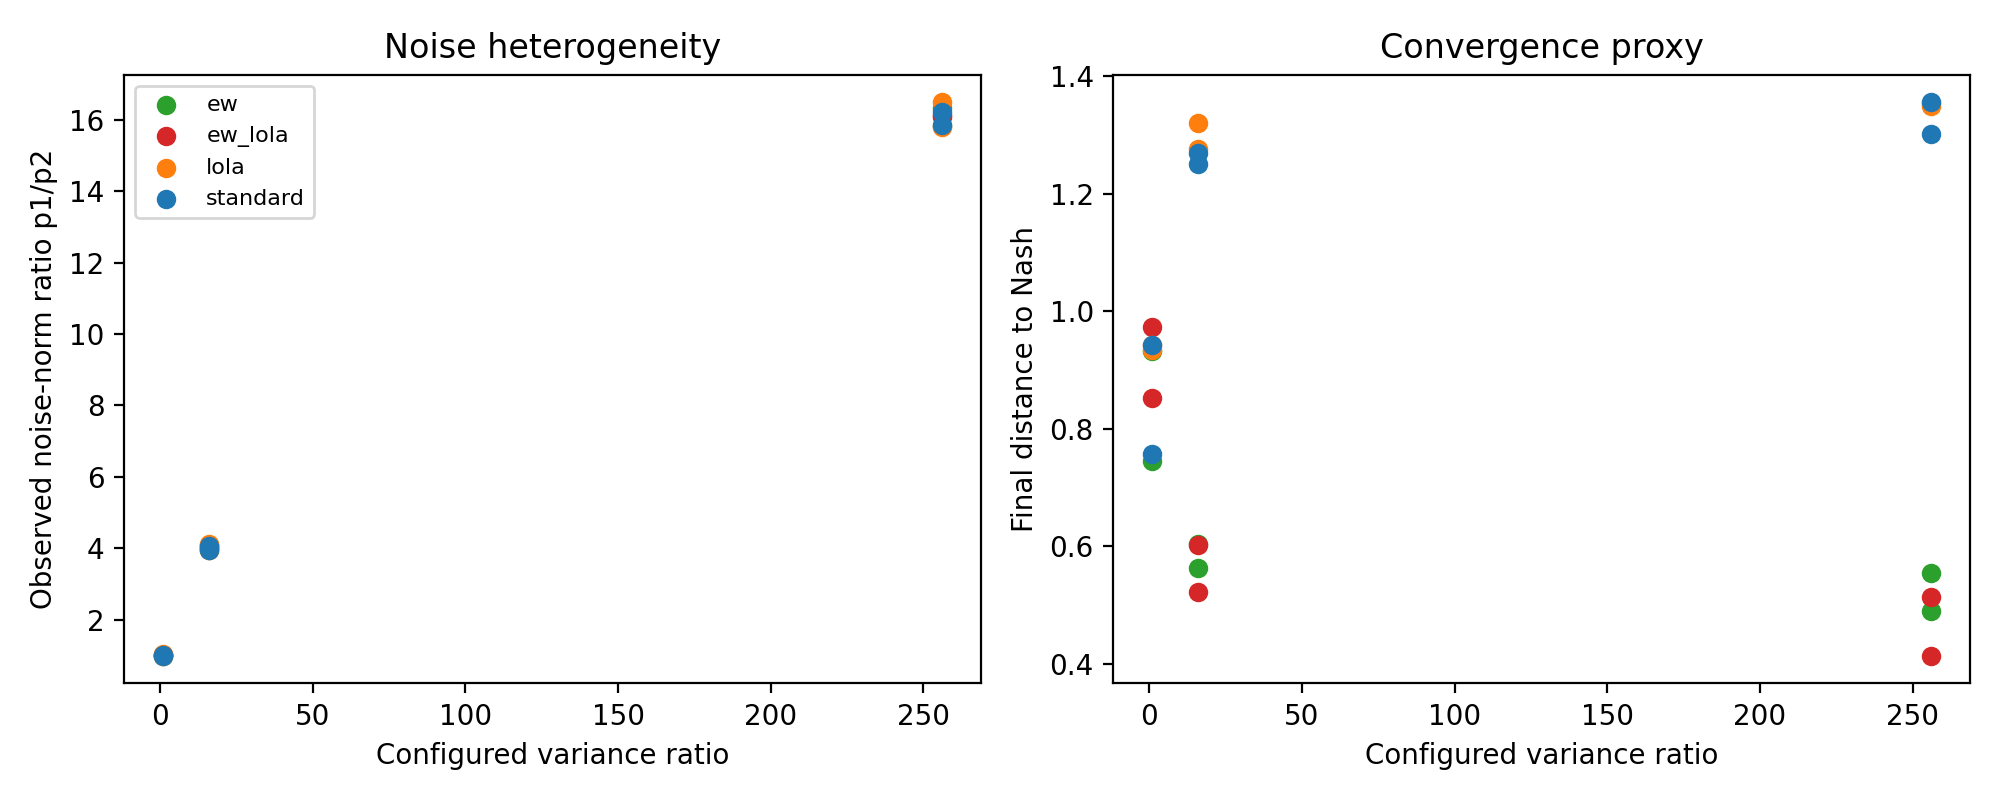
\includegraphics[width=\linewidth]{experiments/artifacts/medium_matrix/matrix_summary.png}
}{
  \fbox{\begin{minipage}{0.94\linewidth}\small
  \textbf{Figure 2 placeholder.}

  Matrix-game variance and convergence proxy. Left: noise heterogeneity versus observed variance proxy under \texttt{standard}, \texttt{ew}, \texttt{lola}, and \texttt{ew\_lola}. Right: final distance-to-Nash proxy versus heterogeneity level.
  \end{minipage}}
}
\caption{Current exploratory matrix-game output. The completed medium sweep already shows that under asymmetric noise, EW-LOLA combines the stability gains of evidence weighting with the shaping gains of LOLA. The final submission should replace this exploratory figure with a paper-ready version built from the same artifact family.}
\label{fig:matrix}
\end{figure}

The current completed sweep is saved in the repository artifacts. In the present scaffold, EW-LOLA is best under heterogeneous noise on both matching pennies and rock-paper-scissors, while pure LOLA degrades sharply in the most asymmetric settings. These runs validate the oracle AM-HM story, not the online estimator story; the latter still needs a separate plug-in-weight ablation.

\subsection{Basin Enlargement in Matching Pennies}

This experiment is the key empirical test for Theorem~\ref{thm:lola-basin}. We therefore use a theorem-facing setup: deterministic matching-pennies dynamics, symmetric logit initialisations around the mixed Nash point, and constant $\lambda$ so that the geometric effect is visible without annealing it away. The relevant quantity is local initialisation sensitivity near the target Nash point, not a global notion of basin volume.

\begin{figure}[t]
\centering
\IfFileExists{experiments/artifacts/basin_matrix/basin_map.png}{
  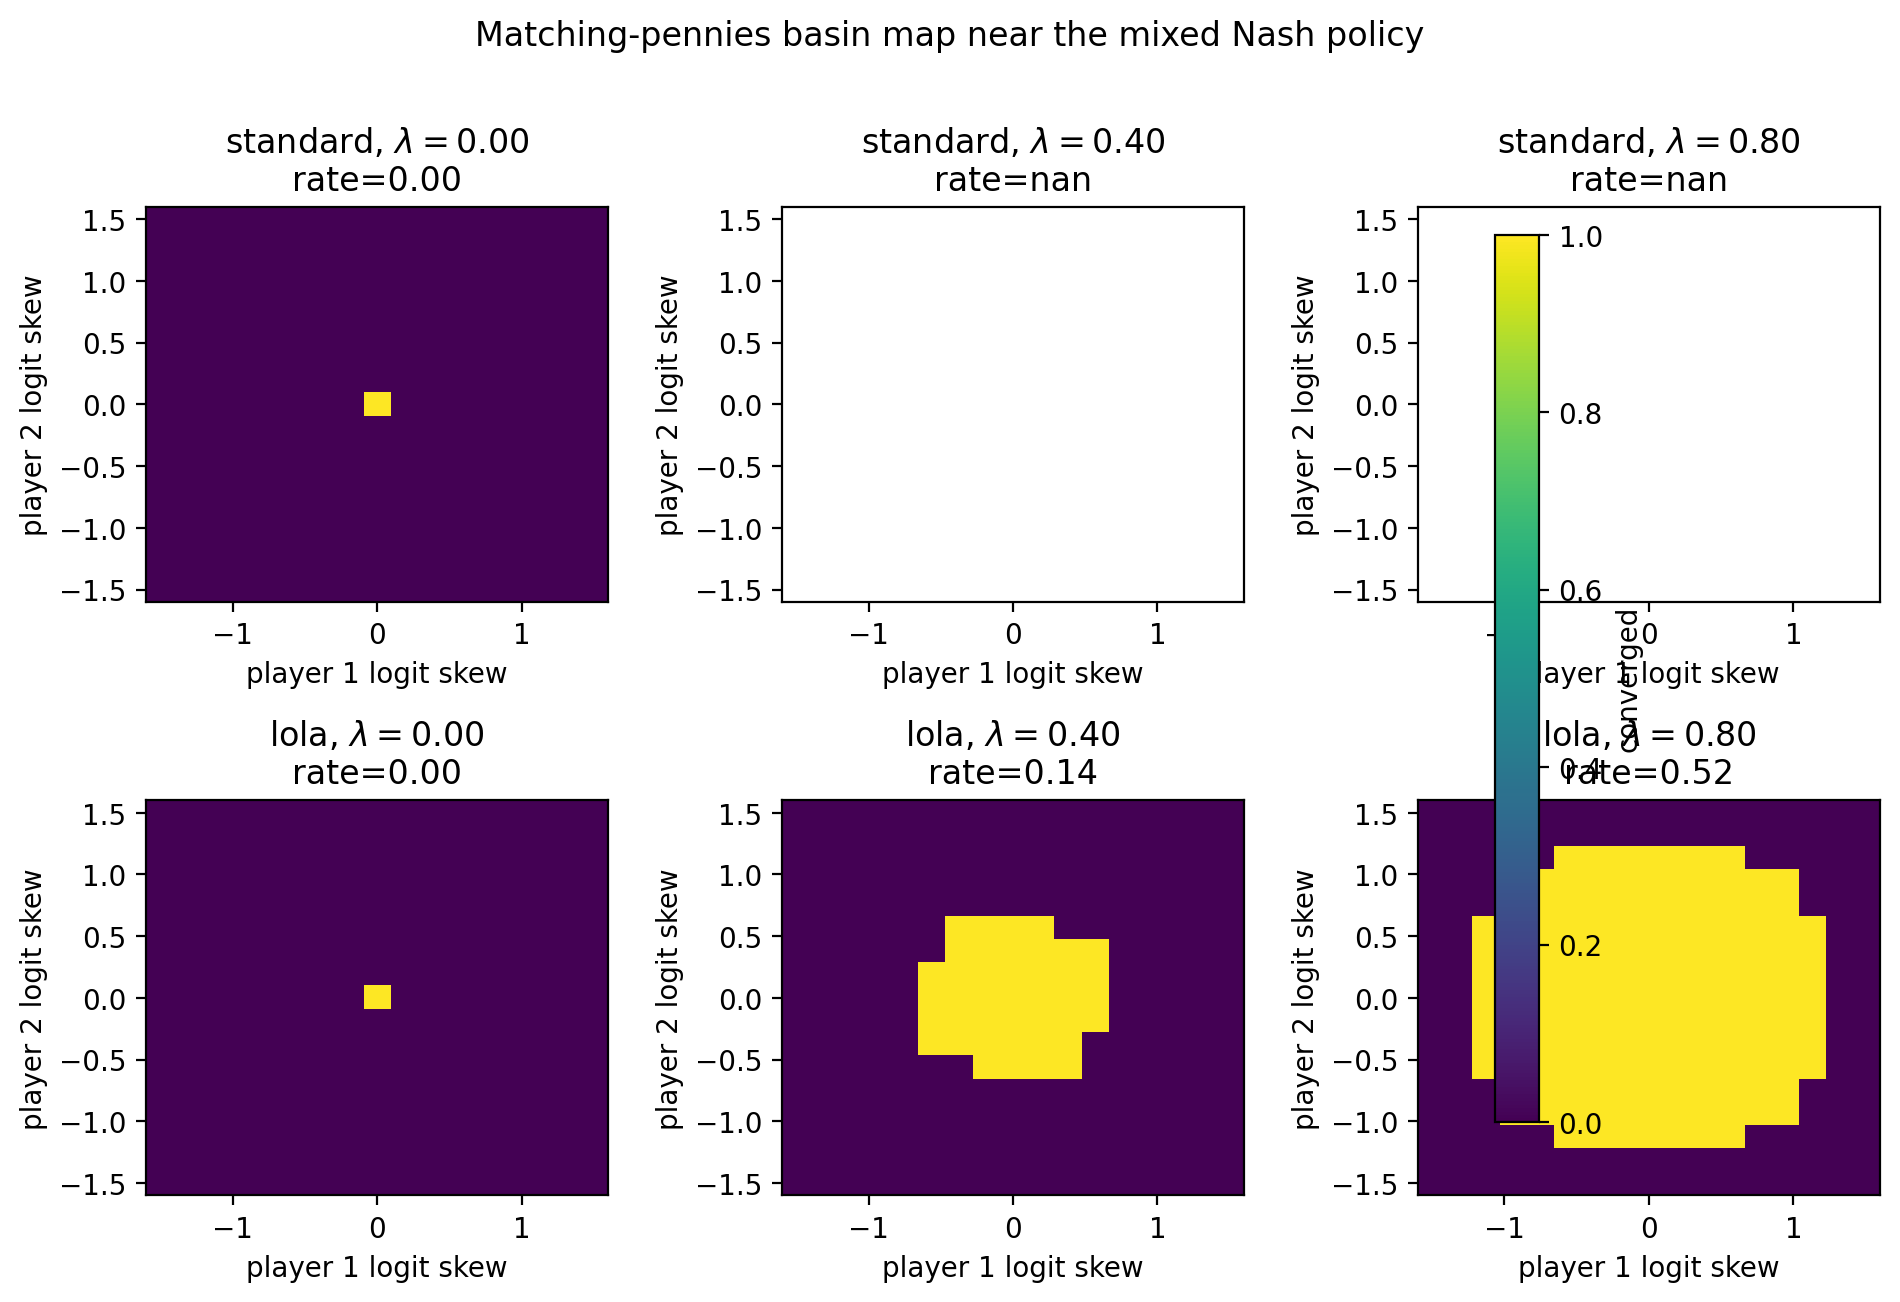
\includegraphics[width=\linewidth]{experiments/artifacts/basin_matrix/basin_map.png}
}{
  \fbox{\begin{minipage}{0.94\linewidth}\small
  \textbf{Figure 3 placeholder.}

  Matching-pennies basin map over symmetric logit initialisations. Standard PG converges only in a very small neighbourhood of the mixed Nash policy, while larger constant-$\lambda$ LOLA enlarges the convergent set.
  \end{minipage}}
}
\caption{Completed basin-mapping diagnostic on matching pennies. On a $17\times 17$ grid of symmetric initialisations in $[-1.6,1.6]^2$, the convergence rate rises from $0.3\%$ for standard PG to $14.2\%$ for LOLA with $\lambda=0.4$ and $51.6\%$ for LOLA with $\lambda=0.8$. This is a local geometry experiment for Theorem~\ref{thm:lola-basin} rather than an asymptotic annealing test.}
\label{fig:basin}
\end{figure}

The main qualitative pattern is the one predicted by the spectral argument: in the rotational zero-sum game, standard PG almost always orbits instead of contracting, whereas constant-$\lambda$ LOLA opens up a visibly larger convergent region. The experiment does not identify a universal best $\lambda$, and it should not be read as a recommendation to keep shaping constant asymptotically. Its role is narrower and cleaner: it validates the local basin-enlargement claim in the game class where the spectral reinforcement condition is expected to hold.

\subsection{Composition in Persona-Conditioned Iterated Games}

This experiment isolates the composition theorem on adaptive game families from \citet{kim2021meta}. The persona-conditioned experiment path is implemented, and the IPD persona sweep is complete in the current scaffold. The matching iterated-RPS persona campaign remains pending because the current LOLA correction uses nested finite differences through the stateful policy and needs optimisation before longer runs become practical. These experiments test adaptation under opponent learning, not the spectral reinforcement condition directly; the basin theorem should therefore not be claimed on the basis of the persona runs alone.

\begin{figure}[t]
\centering
\IfFileExists{experiments/artifacts/medium_kim_ipd/kim_persona_summary.png}{
  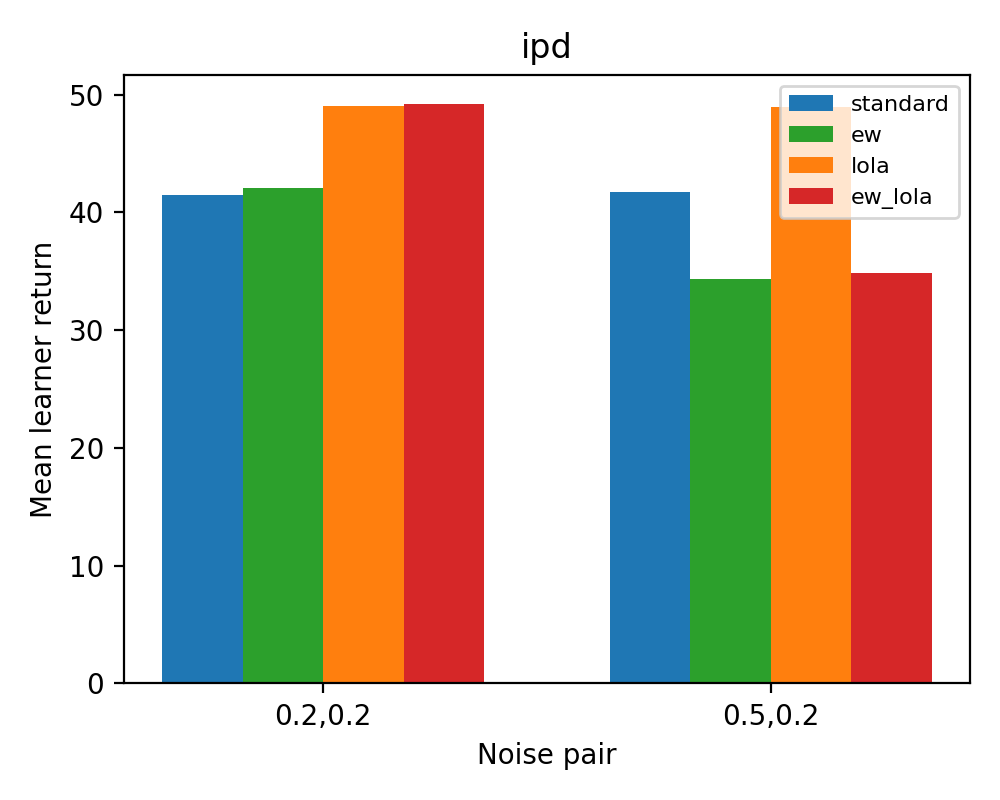
\includegraphics[width=\linewidth]{experiments/artifacts/medium_kim_ipd/kim_persona_summary.png}
}{
  \fbox{\begin{minipage}{0.94\linewidth}\small
  \textbf{Figure 4 placeholder.}

  Persona-conditioned iterated prisoner's dilemma summary. The expected pattern is that EW-LOLA matches LOLA's exploitative advantage while reducing performance collapse in the lower-noise regime.
  \end{minipage}}
}
\caption{Completed Kim-style persona-conditioned IPD sweep. Against adaptive cooperative and defective personas, EW-LOLA is strongest in the lower-noise setting, while pure LOLA is strongest when player~1 is much noisier. The main takeaway is compositional rather than universal dominance: evidence weighting helps in the regime where estimator noise matters, while opponent shaping still carries the exploitative signal against adaptive opponents.}
\label{fig:kim-ipd}
\end{figure}

The current IPD run is enough to show that the composition theorem has a meaningful behavioural test beyond symmetric self-play. It is not yet enough to support a broad claim across all iterated games, which is why the competitive RPS persona campaign remains listed as follow-up work rather than silently folded into the caption.

\subsection{Scaling to N Players}

Following \citet{kim2021meta}, the final workshop version should include a modest scaling check for $N=2,3,4$ iterated RPS. This slot remains unfilled in the current scaffold.

\placeholderfigure{Figure 5 placeholder.}{
Mean return gap between each method and the standard baseline for $N=2,3,4$ iterated RPS. The target claim is modest: EW-LOLA should remain competitive as the number of learners increases.
}{Planned N-player scaling figure. If runtime becomes a problem, it is better to keep $N=2,3,4$ only and treat anything larger as follow-up work.}

\paragraph{Experimental scope.}
The experiment suite is intentionally limited to the tasks that map most directly onto the theory. Matrix games test the AM-HM prediction. Iterated prisoner's dilemma and iterated RPS test shaping and composition under adaptive play. The N-player extension checks whether the combined method remains effective outside the two-player case.

\paragraph{Current experiment status.}
The completed and partially completed experiments are tracked in the repository working notes. A completed matrix sweep, a completed matching-pennies basin map, and a completed Kim-persona IPD sweep are already available, while the iterated-RPS persona and N-player runs remain placeholders in the present draft.

\section{Lean 4 Formalisation}

A companion Lean 4 development formalizes the algebraic backbone of this paper in three files of roughly nine hundred lines total: \texttt{EvidenceWeightedPG.lean} for the energy inequality, the AM--HM bound (Lemma~\ref{lem:amhm}), and the variance-ratio algebra; \texttt{OpponentShapingPG.lean} for bias absorption, annealing compatibility, and the basin-enlargement drift identity (Theorem~\ref{thm:lola-basin}); and \texttt{CooperativePG.lean} for cooperative extensions that are outside the scope of this paper.

The machine-checked portion is the algebraic backbone: AM--HM identities, weight normalisation, and parts of the local linear algebra around shaping. The full stochastic-approximation theorems --- including the final convergence statements for EW-PG, the basin enlargement, and the composition theorem (Theorem~\ref{thm:ewlola}) --- are not yet fully discharged and still carry \texttt{sorry} annotations where current Mathlib support is thin. The Lean files are therefore presented as proof hygiene for the supporting algebra, not as a claim that the headline theorems are machine-checked end-to-end.

\section{Discussion and Limitations}

The contribution is local in four senses. First, the convergence guarantee is local because it inherits the \citet{giannou2022convergence} theorem. EW-LOLA-PG does not solve global equilibrium selection. Second, the basin-enlargement theorem depends on a weighted spectral reinforcement condition that must be checked game-by-game and may fail in potential-like settings. Third, the current variance theorem is for oracle or locally frozen weights; an online-weight theorem and ablation remain open. Fourth, the experiments are still centred on matrix and iterated-game settings. They test the theory cleanly, but they do not yet show performance in deep MARL.

Those limitations are acceptable for this venue if they are stated directly. The paper works best as a compositional theory paper with a compact empirical validation suite. There is also a useful relation to \citet{kim2021meta}. Meta-MAPG models own-learning and peer-learning gradients across a chain of policy updates. EW-LOLA-PG studies local convergence and estimator design for one-step shaping. Kim's iterated-game benchmarks remain valuable because they stress the adaptation dynamics where opponent shaping matters. A separate empirical comparison against strong variance-reduction baselines such as COMA is also still missing, so the present novelty claim is orthogonality rather than blanket superiority over all variance-reduced MARL methods.

\section{Conclusion}

\citet{giannou2022convergence} provided a local convergence theorem for policy gradient in general stochastic games. The Omega technical report added two orthogonal modifications to that picture: evidence weighting, which reduces variance, and opponent shaping, which preserves convergence under annealing and enlarges the local attraction region under constant shaping \citep{shcherbinin2026omega}. This paper isolates those two pieces, proves that their composition can be stated without ambiguity by separating asymptotic convergence from local geometry, and tests the resulting predictions on a compact set of matrix and iterated-game benchmarks. The resulting claim is simple: in local stochastic-game policy optimisation, variance control and opponent shaping can be combined in a mathematically disciplined way.

\appendix

\section{Proof Roadmap for Theorem~\ref{thm:ewlola}}\label{app:proof}

This appendix records the proof structure used repeatedly in Sections~\ref{sec:prelim}--\ref{sec:composition}. It is not a full measure-theoretic reproduction of \citet{giannou2022convergence}; rather, it isolates exactly where the EW and LOLA modifications enter the local recursion.

\paragraph{Step 1: Localized Lyapunov recursion.}
Set $D_n := \|\pi_n-\pi^\ast\|^2$ and work on the localization event $\mathcal{E}_\varepsilon$ that all iterates remain in the neighbourhood $\Omega$ from Assumption~\ref{as:composition}. The projection step and the smoothness of $v$ imply the standard expansion
\begin{equation}\label{eq:appendix-recursion}
\begin{aligned}
\E[D_{n+1}\mid\mathcal{F}_n]
\le\;& D_n\\
&+ 2\gamma_n\langle W_n(v(\pi_n)+\lambda_n\OS(\pi_n)),\,\pi_n-\pi^\ast\rangle\\
&+ C_1\gamma_n B_n\\
&+ C_2\gamma_n^2 \sum_{i=1}^N w_{i,n}^2V_{i,n},
\end{aligned}
\end{equation}
for structural constants $C_1,C_2>0$.

\paragraph{Step 2: Weighted baseline drift.}
Assumption~\ref{as:composition}\textup{(A1)} gives
\[
\langle W^\ast v(\pi_n),\,\pi_n-\pi^\ast\rangle \le -\mu_W D_n.
\]
Using \textup{(A6)} and the Lipschitz continuity from \textup{(A4)}, replacing $W_n$ by $W^\ast$ changes the drift only by $O(D_n^{3/2})$, which can be absorbed into the local remainder term after shrinking $\Omega$ if necessary.

\paragraph{Step 3: Annealed shaping enters as bias, not as asymptotic drift.}
From Assumption~\ref{as:composition}\textup{(A4)},
\[
\OS(\pi_n)=H(\pi_n-\pi^\ast)+O(\|\pi_n-\pi^\ast\|^2).
\]
Under annealing, the term $2\gamma_n\lambda_n\langle W_n\OS(\pi_n),\pi_n-\pi^\ast\rangle$ is of order $O(\gamma_n\lambda_n D_n)$ and therefore summable because $p+r>1$. This is why it can be absorbed into the bias budget in exactly the same way as in Theorem~\ref{thm:lola-rate}. For the \emph{constant}-shaping frozen-weight dynamics, the same term becomes a permanent drift correction, which is the content of Proposition~\ref{prop:ewlola-geometry}.

\paragraph{Step 4: EW modifies only the variance forcing.}
By Lemma~\ref{lem:amhm},
\[
\sum_{i=1}^N w_{i,n}^2V_{i,n}
\le
\frac{\HM(V_n)}{\AM(V_n)} \sum_{i=1}^N V_{i,n},
\]
where $V_n=(V_{1,n},\ldots,V_{N,n})$. Thus the martingale forcing in~\eqref{eq:appendix-recursion} is smaller than in standard PG by the AM--HM factor.

\paragraph{Step 5: No leading mixed term appears.}
The potentially dangerous interaction term is the one combining EW and LOLA. In the localized recursion it is always multiplied by both $\gamma_n$ and $\lambda_n$, hence of order $O(\gamma_n\lambda_n D_n)$ or smaller. Because $p+r>1$, these terms are summable and do not alter the rate exponent.

\paragraph{Step 6: Discrete Gr\"onwall and rate extraction.}
Collecting the previous steps, one obtains
\[
\E[D_{n+1}\mid\mathcal{F}_n]
\le
(1-\gamma_n\mu_W)D_n
+ \widetilde C_1 \gamma_n n^{-\min(\ell_b,r)}
+ \widetilde C_2 \gamma_n^2 \frac{\HM(V)}{\AM(V)}.
\]
Applying the same Chung-type comparison argument used in Proposition~\ref{prop:giannou} yields
\[
\E[D_n\mid \mathcal{E}_\varepsilon]
=
O\!\left(\frac{\HM(V)}{\AM(V)}\cdot \frac{C}{n^q}\right),
\quad
q=\min(\ell_b,p-2\ell_\sigma).
\]
This proves Theorem~\ref{thm:ewlola}.

\section{Planned Large-Scale Extension}

The workshop paper should remain centred on theory-facing validation, but it is worth reserving one appendix slot for a larger benchmark extension. The current staged roadmap moves from theorem-facing matrix and persona-conditioned runs to one medium benchmark family such as PettingZoo or MAgent2, and then to one flagship large-scale suite, preferably Melting Pot for social generalisation or SMACv2 for cooperative micromanagement.

\placeholderfigure{Appendix Figure A1 placeholder.}{
Aggregate scores on one medium-scale benchmark family and one flagship suite, reported with seed variance and instability statistics in addition to mean return.
}{Planned large-scale benchmark extension. The goal is not to benchmark every environment family, but to show that the same qualitative EW-LOLA story survives in at least one serious modern MARL suite.}

\bibliography{references}
\bibliographystyle{icml2026}

\end{document}
